\documentclass[12pt,a4paper]{article}

\usepackage[utf8]{inputenc}
\usepackage[french]{babel}
\usepackage{tikz}
\usepackage[T1]{fontenc}
\usepackage{amsmath}																				% les maths
\usepackage{amsfonts}
\usepackage{amssymb}
\usepackage{fourier}																					% symboles intégral propre
\usepackage{graphicx}
\usepackage[left=2cm,right=2cm,top=2cm,bottom=2cm]{geometry}	% les marges
\usepackage{multicol}																					% pour écrire sur plusieurs colones
\usepackage[thinspace,thinqspace,amssymb]{SIunits}							% écriture des nombres et unités
\usepackage{setspace}																				% set space between lines
\usepackage{enumitem}																				% resume command in enumerate
\usepackage{array}																						% stretch array lines
%\usepackage{url}																							%
\usepackage[breaklinks]{hyperref}															% clickable links
\usepackage[hyphenbreaks]{breakurl}														% for long urls
\usepackage{chemfig}																					% pour les formules chimiques

\hypersetup{
    colorlinks=true,
    linkcolor=red_f,
    citecolor=bleu_f,
    filecolor=green_f,
    urlcolor=bleu_f
}

\usepackage{xcolor}																			% colors
\usepackage[framemethod=tikz]{mdframed}									% fancy environments

%%%%%%%%%% graphic charter

\renewcommand{\familydefault}{\sfdefault}												% sans serif font

%%%%% HEADER
%\pagestyle{fancy}
%\lhead{\textcolor{gray_f}{Physique-Chimie\\R. METZDORFF}}
%\chead{\textcolor{gray_f}{Lycée Suzanne Valadon}}
%\rhead{\textcolor{gray_f}{2020-2021}}
%\renewcommand{\headrulewidth}{0.4pt}
%\let\HeadRule\headrule
%\renewcommand\headrule{\color{gray_f}\HeadRule}

%%%%% COLORS
\definecolor{gray_f}{RGB}{68,84,106}
\definecolor{gray_c}{RGB}{214,220,229}
\definecolor{gray_cc}{RGB}{245,245,245}
\definecolor{bleu_f}{RGB}{91,155,213}
\definecolor{bleu_c}{RGB}{222,235,247}
\definecolor{red_f}{RGB}{204,0,0}
\definecolor{red_c}{RGB}{245,204,204}
\definecolor{orange_f}{RGB}{237,125,49}
\definecolor{orange_c}{RGB}{251,229,214}
\definecolor{green_f}{RGB}{112,173,71}
\definecolor{green_c}{RGB}{226,240,217}
\definecolor{yellow_f}{RGB}{255,192,0}
\definecolor{yellow_c}{RGB}{255,242,204}
\definecolor{code_keyword}{RGB}{23,23,139}										% colors for pyhton code
\definecolor{code_comment}{RGB}{50,137,21}
\definecolor{code_string}{RGB}{139,139,25}
\definecolor{red_unilim}{RGB}{166,41,41}
\definecolor{gray_unilim}{RGB}{78,87,94}
\definecolor{orange_unilim}{RGB}{209,98,40}

%%%%% NEW ENVIRONMENTS

%%% header
\mdfdefinestyle{s_head}{%
	linecolor=red_unilim!,
	outerlinewidth=3pt,%
	frametitlerule=false,
	topline=false,
	bottomline=false,
	rightline=false,
	leftline=false,
	backgroundcolor=red_unilim,
	innertopmargin=8pt,
	roundcorner=0pt,
	nobreak=true,
	fontcolor=white
}
\newmdenv[style=s_head]{header_env}
\newenvironment{header}
{%\stepcounter{exa}%
	\addcontentsline{ldf}{figure}{0}%
	\begin{header_env}\qquad\Large\bf}
	{\end{header_env}}

%%%%% New command

\newcommand{\app}{\colorbox{bleu_c}{\textcolor{bleu_f}{APP}}}
\newcommand{\rea}{\colorbox{yellow_c}{\textcolor{yellow_f}{REA}}}
\newcommand{\anarai}{\colorbox{green_c}{\textcolor{green_f}{ANA-RAI}}}
\newcommand{\val}{\colorbox{orange_c}{\textcolor{orange_f}{VAL}}}
\newcommand{\com}{\colorbox{red_c}{\textcolor{red_f}{COM}}}
\newcommand{\auto}{\colorbox{white}{\textcolor{black}{AUTO}}}
\newcommand{\rco}{\colorbox{gray_c}{\textcolor{gray_f}{RCO}}}


\bibliographystyle{custom-bib/thesis}
\usepackage{bibentry}
\usepackage{pdfpages}

\title{L'expérience de Benjamin Franklin... Et Rayleigh, Pockels, Devaux, et Langmuir}
\author{Rémi Metzdorff}
\date{\today}

\begin{document}

%\maketitle

\begin{header}
\begin{minipage}{0.55\textwidth}
Rapport de Master 2
\end{minipage}
\begin{minipage}{0.38\textwidth}
\href{https://www.unilim.fr/}{
\includegraphics[scale=1]{logo.png}}
\end{minipage}
\end{header}

\vspace{30pt}
\begin{spacing}{1.2}
{\bf
\begin{Large}
\noindent
\textcolor{gray_unilim}{INSPE Académie de Limoges}
\end{Large}

\begin{large}
\noindent
\textcolor{gray_unilim}{Métiers de l'enseignement, de l'éducation et de la formation}

\noindent
\textcolor{orange_unilim}{Master MEEF Second degré}

\noindent
\textcolor{orange_unilim}{Professeur de Physique et de Chimie}
\end{large}
}

\vspace{20pt}

\noindent
\textcolor{gray_unilim}{2020--2021}

\vspace{40pt}
\begin{large}
\bf
\noindent
\textcolor{orange_unilim}{Mesurer une molécule d'huile avec Benjamin Franklin, lord Rayleigh, Agnes Pockels,  Henri Devaux, Irving Langmuir, etc.}

\vspace{150pt}
\noindent
\textcolor{gray_unilim}{Rémi Metzdorff}

\noindent
\textcolor{orange_unilim}{Lycée Suzanne Valadon}
\end{large}
\end{spacing}

\vfill

\hfill

\includegraphics[scale=1]{logo_bottom.png}

\thispagestyle{empty}

\newpage

\tableofcontents
\newpage

\section*{Introduction}
\addcontentsline{toc}{section}{Introduction}

Vers la fin du XVIII\textsuperscript{ème} siècle, Benjamin Franklin verse une petite cuillère d'huile dans un étang près de Londres.
Il remarque que la tache d'huile s'étend rapidement à la surface jusqu'à recouvrir une bonne partie du plan d'eau.
En divisant le volume d'huile renversé par la surface recouverte, on trouve l'épaisseur de la tache d'huile qui s'avère être de l'ordre du nanomètre, c'est à dire la taille d'une molécule d'huile.
Mais ce n'est pas Franklin qui eu l'idée de ce calcul.
Lui avait d'autres préoccupations à son époque.

L'expérience est belle : en mesurant deux quantités réellement macroscopiques, on accède à la taille caractéristique d'un des plus petits constituants de la matière.
Il y a quelques années, elle était couramment reproduite à petite échelle au lycée et il existe de nombreuses ressources et activités sur le sujet.
Par exemple, on peut trouver plusieurs articles du bulletin de l'union des physiciens (BUP) sur ce thème \cite{Carron1992, Schwob2000, Bacciochini2002, Serra2002}.
L'expérience est toutefois plus subtile qu'il n'y parait peut-être, ce qui explique à la fois son interprétation tardive et les difficultés rencontrées parfois pour la reproduire.

\section{L'expérience historique et son interprétation}

Le billet de blog de David Louapre~\cite{Louapre2012} constitue une bonne introduction au sujet.
À sa lecture on se rend bien compte qu'attribuer tout le mérite de cette expérience à Benjamin Franklin est un peu exagéré.
C'est grâce à un article du bulletin de l'union des physiciens~\cite{Bolmont2001} que j'ai pu orienter mes recherches sur les différents auteurs ayant contribué à la compréhension de cette expérience et cibler les articles utiles.

\subsection{Benjamin Franklin (1706--1790)}

L'expérience est relatée par Benjamin Franklin lui même dans une lettre adressée à William Brownrigg\cite{Franklin1773a} :
\begin{itemize}
\item[]
\og
At length being at Clapham where there is, on the common, a large pond, which I observed to be one day very rough with the wind, I fetched out a cruet of oil, and dropped a little of it on the water.
I saw it spread itself with surprising swiftness upon the surface ;
[...] the oil, though not more than a tea spoonful, produced an instant calm over a space several yards square, which spread amazingly and extended itself gradually till it reached the lee side, making all that quarter of the pond, perhaps half an acre, as smooth as a looking-glass.
\fg{}.
\end{itemize}
Le reste de la lettre montre que la préoccupation de Franklin n'est pas la mesure de la taille des molécules d'huile.
Lui s'intéresse plutôt au calme produit par l'huile sur une surface d'eau agitée par le vent~\cite{Mertens2006}.

\subsection{Lord Rayleigh (1842--1919) et Agnes Pockels (1862--1935)}

Il faut attendre la fin du XIX\textsuperscript{ème} siècle pour que Rayleigh reprenne le principe de cette expérience et en déduise l'épaisseur de la couche d'huile~\cite{Rayleigh1890a}.
Pour cet article, il mesure\footnote{Avec une balance précise au vingtième de milligramme !} la masse d'huile d'olive nécessaire pour stopper le mouvement de copeaux de camphre\footnote{À cette époque, il semble que le camphre soit couramment utilisé comme indicateur de la valeur de la tension de surface de l'eau.
Dans un autre article~\cite{Rayleigh1892}, on peut lire que si la tension de surface d'une eau contaminée diminue en dessous de 0{,}72 fois celle d'une surface propre, le camphre ne bouge plus.
Si on prend la valeur d'une interface eau-air à \unit{20}{\celsius} ($\gamma_\mathrm{eau-air}=\unit{72{,}8}{\milli\newton\per\meter}$), on trouve une valeur seuil de \unit{52{,}4}{\milli\newton\per\meter} appelée \og camphor point \fg{} .
La précision de cette valeur est remise en question plus tard par Rayleigh qui proposera \cite{Rayleigh1899} 0{,}78 au lieu de 0{,}72 donnant un point camphre de \unit{56{,}8}{\milli\newton\per\meter}.
C'est cette dernière valeur qui est retenue pour reproduire la figure~\ref{fig:rayleigh99}.} à la surface d'une bassine d'eau.
D'après la masse volumique de l'huile, il calcule le volume d'huile déposé à la surface de l'eau et, connaissant la surface de la bassine, il calcule l'épaisseur de la couche d'huile nécessaire pour immobiliser le camphre et trouve une valeur de l'ordre du nanomètre :
\begin{itemize}
\item[]
\og
The thickness of oil required to take the life out of the camphor movements lies between one and two millionths of a millimetre, and may be estimated with some precision at 1{.}6 micro-millimetre.
\fg{}.
\end{itemize}

Les expériences menées par Agnes Pockels~\cite{Pockels1891, Pockels1894} permettent d'améliorer ces mesures.
Elle propose de diluer l'huile dans un solvant volatil (le benzène) pour en introduire une quantité très faible à la surface d'un récipient d'eau et met en place un dispositif expérimental permettant de faire varier la surface d'une interface eau-air contaminée.

\begin{figure}
\center
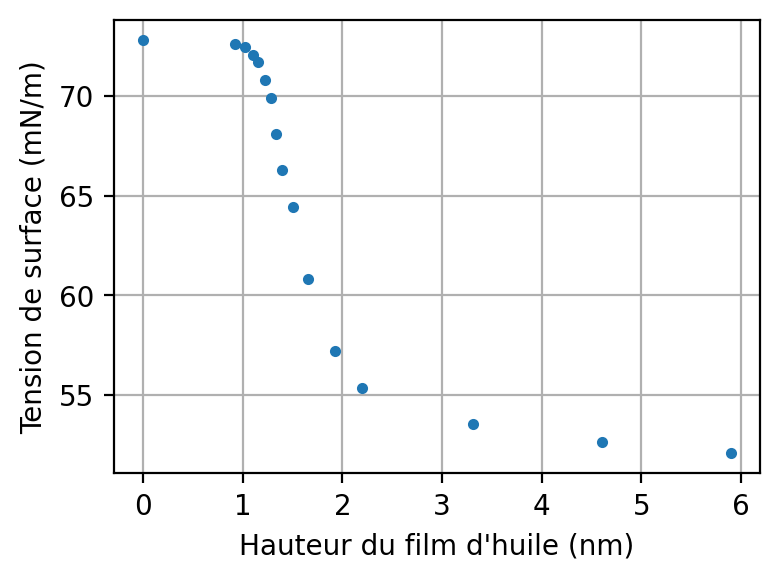
\includegraphics[scale=1]{rayleigh99.png}
\caption{Évolution de la tension de surface d'une interface eau-air contaminée par de l'huile de castor, en fonction de la hauteur du film d'huile calculée comme s'il était continu.
On remarque que : la tension superficielle reste constante pour une épaisseur inférieure à \unit{1}{nm} et quasi-constante au delà de \unit{2}{nm}.
D'après les données de \cite{Rayleigh1899}.}
\label{fig:rayleigh99}
\end{figure}

En 1899, Rayleigh réitère donc son expérience à l'aide d'un nouveau dispositif inspiré de celui de Pockels :
\begin{itemize}
\item[]
\og 
The water is contained in a trough modelled after that of Miss Pockels.
It is of tin-plate, \unit{70}{cm} long, \unit{10}{cm} broad, and \unit{2}{cm} deep, and it is filled nearly to the brim.
The partitions, by which the oil is confined, are made of strips of glass resting upon the edge of the trough in such a manner that their lower surfaces are wetted while the upper surfaces remain dry.
\fg{}
\end{itemize}
Après avoir introduit une quantité mesurée d'huile diluée à la surface de ce dispositif, il peut donc faire varier la \og densité \fg{}\footnote{Pour reprendre les termes de l'article.
Il serait peut-être plus judicieux de parler de concentration surfacique comme suggéré par les remarques de Pockels \cite{Pockels1891}.} d'huile en modifiant l'aire de l'interface.
Pour différentes valeurs de densité, il mesure la tension superficielle à l'aide d'une balance de Wilhelmy.
Finalement on peut calculer la hauteur du film d'huile comme s'il était continu en comparant la quantité d'huile introduite et la surface disponible comme précédemment.

Avec les données de l'article, on peut tracer l'évolution de la tension superficielle d'une interface contaminée en fonction de la hauteur du film d'huile (Fig.~\ref{fig:rayleigh99}).
\footnote{Les valeurs exactes des tensions de surface et de l'épaisseur du film d'huile sont sujettes à caution.
En particulier, elles sont différentes de celles de Freundlich \cite{Freundlich1909}, qui devait avoir de très bonnes raisons de tracer la courbe comme il l'a fait, mais elles m'échappent.}
Dans ses conclusions, Rayleigh donne pour la première fois une interprétation moléculaire aux résultats obtenus :
\begin{itemize}
\item[]
\og 
It is obvious therefore that the present phenomena lie entirely outside the scope of a theory such as Laplace's, in which matter is regarded as continuous, and that an explanation requires a direct consideration of molecules.
\fg{} 
\end{itemize}
et en déduit ainsi le diamètre d'une molécule d'huile en supposant la présence d'un film mono-moléculaire :
\begin{itemize}
\item[]
\og 
[...] we conclude that the first drop in tension corresponds to a complete layer one molecule thick, and that the diameter of a molecule of oil is about \unit{1}{nm}.
\fg{} 
\end{itemize}

\subsection{Henri Devaux (1862--1956)}

Au début du XX\textsuperscript{ème} siècle, Devaux s'intéresse aussi à ces expériences et mène ses propres mesures \cite{Devaux1904}.
Le raisonnement mené sur une expérience réalisée plus tardivement reste le même \cite{Devaux1931} :
\begin{itemize}
\item[]
\og On a ainsi la surface moyenne occupée par une lame.
Cette surface était, dans les expériences faites le 18 avril 1912 de \unit{363{,}71}{cm\squared}.
Or, cette surface d'huile a été produite par deux gouttes de la solution, c'est-à-dire par $\unit{400\times10^{-7}}{cm\cubed}$ d'huile.
L'épaisseur de la lame était donc de :
\[
e = \frac{V}{S} = \frac{400\times10^{-7}}{363{,}71} = \unit{1{,}10\times10^{-7}}{cm}
\]
avec une approximation allant de $1{,}04$ à $\unit{1{,}15\times10^{-7}}{cm}$.
On peut donc dire que la plus mince lame d'huile cohérente qui peut exister sur l'eau possède 1{,}1 millionième de millimètre.
\fg{} 
\end{itemize}
Il parvient ainsi à obtenir une valeur de la taille d'une molécule d'huile (l'oléine) de \unit{1{,}1}{nm}, qu'il compare à la valeur théorique calculée sur la base des travaux de Nernst.
L'accord est suffisamment bon pour que la présence de films mono-moléculaires soit confirmée.

Le protocole expérimental est différent \cite{Marcelin1914, Devaux1931} et peut également s'appliquer aux films solides.
Pour l'huile, s'il l'utilise toujours diluée dans du benzène, la mesure de la surface occupée par l'huile est réalisée grâce à du talc saupoudré avant l'introduction de l'huile sur une interface eau-air nettoyée à l'aide de bandelettes de papier (Fig.~\ref{fig:devaux1931}).
C'est probablement cette expérience qui a inspiré les versions de l'expérience de Franklin réalisées en lycée.
\begin{figure}
\center
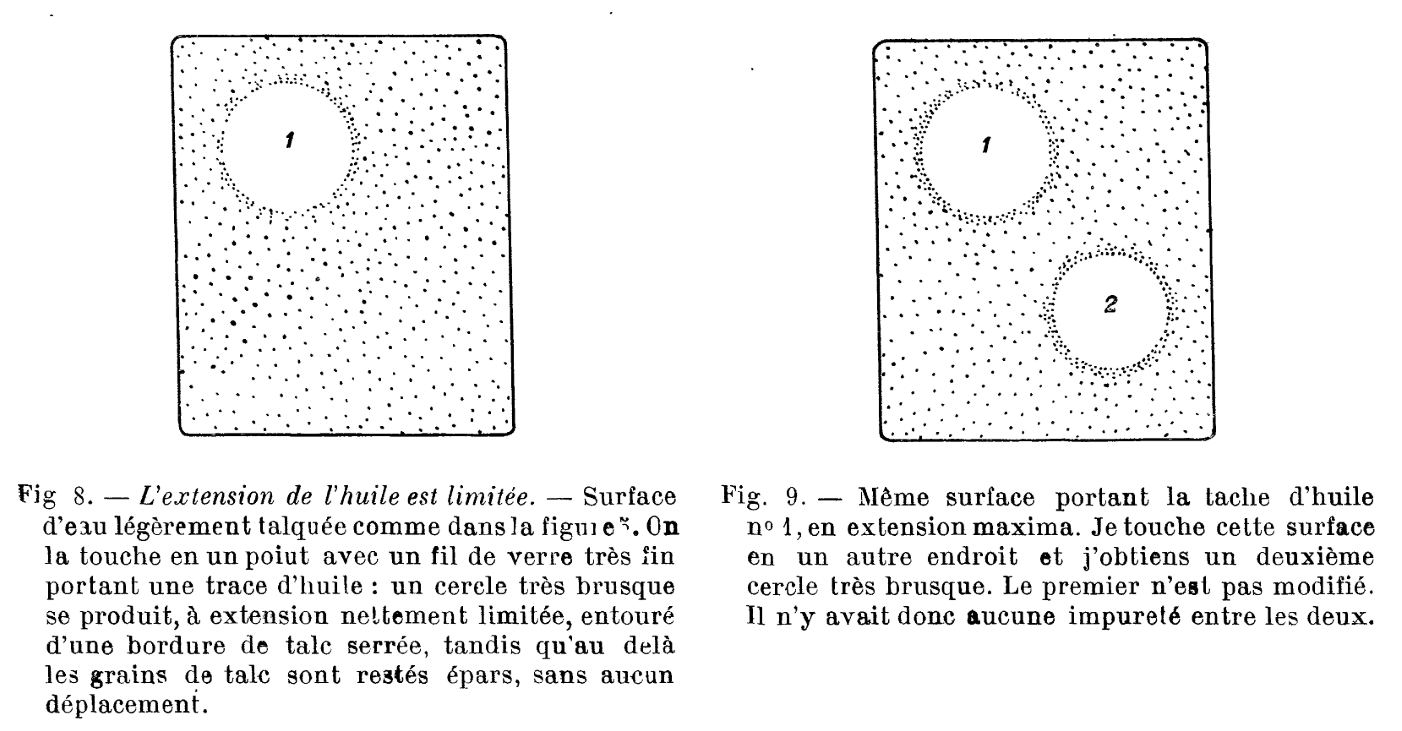
\includegraphics[scale=0.5]{devaux1931a.png}

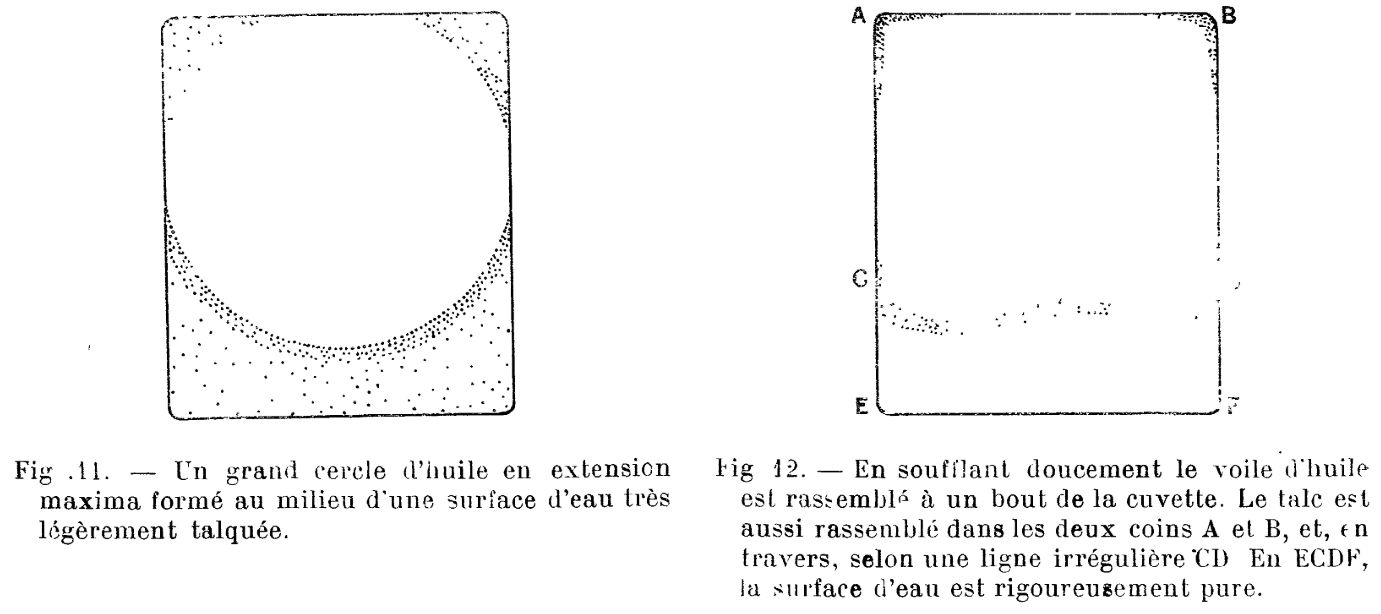
\includegraphics[scale=0.5]{devaux1931b.png}

\caption{Figures issus de \cite{Devaux1931} pour décrire les expériences de Devaux sur l'extension finie d'une quantité d'huile à la surface de l'eau et pour la mesure de la surface occupée par une quantité connue d'huile.}
\label{fig:devaux1931}
\end{figure}

\subsection{Irving Langmuir (1881--1957)}

\begin{figure}
\center
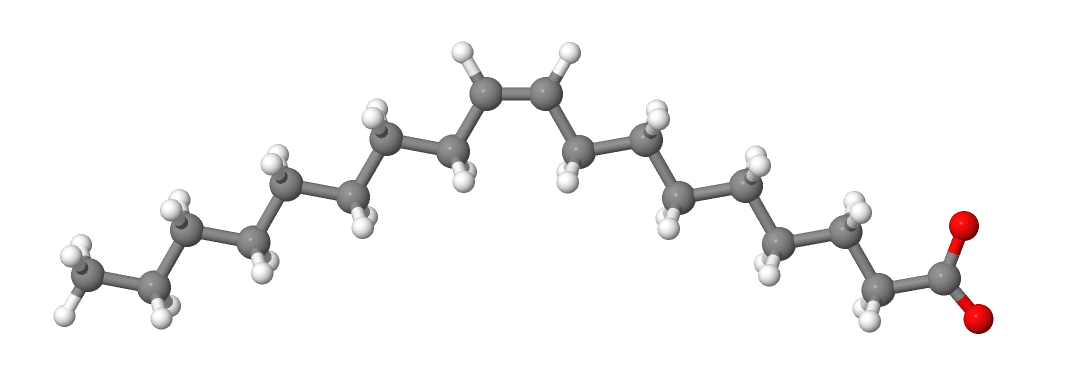
\includegraphics[scale=0.4]{acide_oleique.png}
\caption{Structure d'une molécule d'acide oléique.}
\label{fig:acide_oleique}
\end{figure}

Jusqu'alors, les raisons qui poussent l'huile à s'étendre à la surface de l'eau restent mystérieuses.
C'est Langmuir qui propose une explication théorique \cite{Langmuir1917}.
\footnote{Son article est aussi une excellente revue des différentes contributions présentés jusqu'ici.}
En prenant l'exemple de l'acide oléique (Fig.~\ref{fig:acide_oleique}), il explique l'extension du liquide à la surface de l'eau comme le résultat d'une affinité du groupement carboxyle avec l'eau (tête hydrophile) et d'une affinité des chaines carbonées les unes avec les autres (queue hydrophobe) :
\begin{itemize}
\item[]
\og [...] when oleic acid is placed on water, it is probable that the carboxyl groups do actually dissolve in water; that is, they combine with the water chemically (by secondary valence). The long hydrocarbon chains have too much attraction for each other, however, and too little for water, to be drawn into solution merely because of the affnity of the carboxyl for the water.
[...]
The spreading of an oil upon water is thus due to the presence of an "active group" in the molecule; that is, some group which has a marked affinity (secondary valence) for water.
\fg{} 
\end{itemize}

S'inspirant des travaux de Devaux et Marcelin, il mène ses propres expériences et pousse l'interprétation des résultats encore plus loin pour déterminer la forme des molécules à la surface de l'eau.
Connaissant cette fois le nombre de molécules déposées à la surface de l'eau, il peut calculer la surface occupée par une seule molécule sur l'interface eau-air.
Avec l'acide oléique, il trouve que la dimension latérale de la molécule est environ deux fois plus faible que sa hauteur, ce qui tend à confirmer ses hypothèses.

L'ensemble de ces travaux a ouvert la voie au procédé de déposition Langmuir-Blodgett  qui permet encore actuellement d'obtenir des film mono ou multicouche de composés variés \cite{BiolinScientific2011}.

\section{Proposition d'activité en classe de seconde générale}

La lecture des documents précédemment cités est très éclairante quant à la manière dont l'expérience était traitée et reproduite expérimentalement au lycée.
L'activité présentée dans ce document repose sur un problème ouvert inspiré de l'expérience décrite dans la lettre de Benjamin Franklin~\cite{Franklin1773a}.
Il s'agit d'une approche documentaire, éventuellement mais pas nécessairement étayée par des mesures expérimentales pour déterminer certaines grandeurs non précisées dans le sujet.
L'objectif n'est pas de reproduire l'expérience comme l'ont fait Rayleigh, Pockels, Devaux, Marcelin ou Langmuir.
Cette séquence est divisée en deux temps :
\begin{itemize}
\item l'activité proprement dite où les élèves se confrontent au problème pendant toute la durée d'une séance de TP (1h30).
Le sujet élève de l'activité est présenté en annexe de ce document (Annexe~\ref{ann:sujet}) ;
\item une conclusion en classe entière après que les élèves aient réalisé un travail biographique sur deux des principaux acteurs de cette expérience : Franklin et Rayleigh.
\end{itemize}

\subsection{Dans le programme}

Cette activité rentre dans le cadre de la première partie du thème \og Constitution et transformations de la matière \fg{} et plus particulièrement au début de l'étude de la \og Modélisation de la matière à l'échelle microscopique \fg{}.
Voici l'extrait du programme concerné :
\begin{center}
\begin{tabular}{|l|l|}
\hline
\textbf{Du macroscopique au} 			& Définir une espèce chimique comme une collection d'un \\
\textbf{microscopique, de l'espèce}	& nombre très élevé d'entités identiques. \\
\textbf{chimique à l'entité.}					& \\
																& Exploiter l'électroneutralité de la matière pour associer\\
Espèces moléculaires, espèces		& des espèces ioniques et citer des formules de composés\\
ioniques, électroneutralité de la			& ioniques.\\
matière au niveau	 macroscopique.	& \\
\hline
Entités chimiques : molécules,			& Utiliser le terme adapté parmi molécule, atome, anion et \\
atomes, ions.											& cation pour qualifier une entité chimique à partir d'une \\
																& formule chimique donnée. \\
\hline
\end{tabular}
\end{center}
Le cheminement suggéré dans le programme est ici suivi à la lettre puisque cette expérience nécessite de décrire l'huile d'olive\footnote{Que l'on assimilera à de la trioléine, puisqu'il s'agit de l'espèce largement majoritaire dans l'huile d'olive.} dans un premier temps comme une espèce chimique puis de s'intéresser aux entités chimiques qui la compose.
On part d'un volume macroscopique d'une espèce pour en déduire la taille microscopique des entités correspondantes.

S'agissant d'une tâche complexe, de nombreuses compétences de la démarche scientifique sont mobilisées même si l'attention est plus particulièrement portée sur certaines d'entre elles lors de l'évaluation.

Enfin, cette activité est évidemment une occasion de suivre la recommandation générale du programme concernant la \og mise en perspective des savoirs avec l'histoire des sciences \fg{}.

\subsection{Prérequis}

Les élèves ont déjà été confrontés à des problèmes plus ou moins ouverts notamment lors des séances de TP.
Ce n'est donc pas la première fois qu'ils doivent s'appuyer sur la méthode de résolution dont les étapes sont rappelées dans le sujet.

Dans le chapitre qui précède, les élèves ont revu les termes molécule et atome, les entités qui composent les espèces chimiques.

Pour pouvoir rapprocher l'épaisseur du film d'huile de la taille d'une molécule, les élèves doivent avoir une idée correcte de la taille d'un atome.
Cette valeur a été donnée dans le cours précédent cette activité.
Ils ont aussi fait un exercice consistant à estimer la taille du personnage de la vidéo \href{https://youtu.be/oSCX78-8-q0}{A boy and his atom} en comptant les \og atomes \fg{} qui le composent.
Par analogie, ils peuvent ainsi compter les atomes des chaines carbonées de la trioléine pour émettre leur hypothèse.

La manipulation des puissances de dix ne doit pas être un obstacle majeur lors des applications numériques.
Ceci a été revu également peu de temps avant l'activité.

Certaines capacités expérimentales sont également requises :
\begin{itemize}
\item mesurer un volume à l'aide d'une éprouvette ;
\item mesurer des distances sur un schéma en s'aidant d'une échelle de longueur.
\end{itemize}

\subsection{Objectifs}

\subsection{L'activité}

\subsubsection{Déroulement de la séance}

\paragraph{Accueil (5')}
\begin{itemize}
\item[•] Accueil des élèves, désinfection des mains, placement imposé par trinôme (la composition des groupes est projetée au tableau), \og Bonjour à tous, asseyez-vous. \fg{}
\item[•] Appel.
\item[•] Contextualisation : 

\og Rappelez vous le titre du chapitre 3, du macroscopique au microscopique : on part d'une description de la matière à notre échelle pour en venir à l'étude des particules qui composent la matière.
Avec l'activité d'aujourd'hui c'est exactement le chemin que l'on va suivre : on va interpréter une expérience macroscopique, à notre échelle, pour déterminer la taille d'une molécule d'huile.
On va essayer répondre à la question : Quelle est la taille d'une molécule d'huile ?\fg{}
(la question est écrite au tableau).
\end{itemize}

\paragraph{Présentation de la séance (2')}
\begin{itemize}
\item[•]  \og Tout le monde écoute, je vous donne les consignes générales.\fg{}

\item[•] Consignes :
\begin{itemize}
\item Objectif : répondre à la question \og Quelle est la taille d'une molécule d'huile ? \fg{}
\item \og Vous rédigerez un compte-rendu chacun, j'en ramasserai un par groupe au hasard à la fin. \fg{}
\item \og Servez-vous de l'aide à la rédaction du compte-rendu rappelée dans le sujet.
La première étape sera comme d'habitude de donner votre hypothèse \og Je pense qu'une molécule d'huile mesure ... car ... \fg{}
\end{itemize}

\item[•] \og Est-ce qu'il y a des questions ?
C'est bon pour tout le monde ?

Vous avez quinze minutes pour parcourir le sujet et formuler votre hypothèse.
Appelez moi quand c'est fait.

Je vous distribue le sujet et c'est parti.
\fg{}
\end{itemize}

\paragraph{Préparer la fiche de notation avec le nom des binômes.}

\paragraph{Au bout de quinze minutes, vérifier les hypothèses, puis aide en fonction de chaque groupe.}

\paragraph{Première aide}
\begin{itemize}
\item[•] Coup de pouce : Commencez par déterminer le volume d'une cuillère à café.
\item[•] Aide : Quelle verrerie peut-on utiliser pour mesurer un volume ?
\item[•] Aide : Mesure le volume d'une cac d'huile avec une éprouvette.
\item[•] Aide : Une cac fait 2 mL.
\end{itemize}

\paragraph{Deuxième aide}
\begin{itemize}
\item[•] Coup de pouce : Dessinez la tache d'huile en 3D puiis formule du volume du cylindre.
\item[•] Aide : À quoi correspondent les différentes grandeurs dans la formule, lesquelles sont connues ?
\item[•] Aide : Mesure l'aire sur le schéma
\item[•] Aide : L'aire de la flaque est \unit{2000}{m\squared}
\end{itemize}

\paragraph{Troisième aide}
\begin{itemize}
\item[•] Coup de pouce : Pourquoi la tache arrête-t-elle de s'étendre ?
\item[•] Aide : Ça vous semble normal de trouver un chiffre aussi petit ?
\item[•] Aide : Le professeur verse des haricots sur la table
\item[•] Aide : L'huile forme une couche haute comme une seule molécule
\end{itemize}

\paragraph{Nettoyage}

\paragraph{Ramasser les compte-rendus}
 
\paragraph{Fin de la séance}

\subsubsection{Matériel}

Le matériel est à disposition des élèves mais pas directement sur leur paillasse :
\begin{itemize}
\item[•] bécher \unit{100}{mL} ;
\item[•] éprouvettes graduées \unit{10}{mL} et plus ;
\item[•] balance ;
\item[•] cuillère à café ;
\item[•] entonnoir ;
\item[•] eau ;
\end{itemize}

\subsubsection{Évaluations}

Lors de la séance, l'évaluation est portée sur trois compétences en particulier : analyser-raisonner (\anarai{}), réaliser (\rea{}) et valider (\val{}).\footnote{Puisque l'activité est un problème ouvert, d'autres compétences sont inévitablement mobilisées mais il est possible de les évaluer après la séance sur la base du compte-rendu rédigé par les élèves.
Ce n'est pas sur celles-ci que l'accent est mis pour cette activité.}
Le niveau de maitrise de ces compétences est graduée selon quatre niveaux identifiables d'après l'aide apportée lors de la séance : A (bien maitrisée), B (maitrisée), C (insuffisamment maitrisée) et D (non maitrisée) (Tab.~\ref{tab:cptces_tp}).

Le compte-rendu est aussi évalué sur la base des compétences mobilisées (Tab.~\ref{tab:cptces_cr}).

\begin{table}[p]
\center
\begin{tabular}{l|l|c}
\textbf{Compétence} & \textbf{Aptitude} / Observable & \textbf{Niveau} \\
\hline \hline
\anarai 	& \textbf{Élaborer un protocole qui répond à la question} 	& \\
				& L'élève mesure le volume de 10 cac				 						& A+ \\
				& L'élève mesure le volume d'une cac 									& A \\
				& Aide : Avec quelle verrerie peut-on mesurer un volume ?	& B \\
				& Aide : Mesure le volume d'une cac d'huile avec une éprouvette & C \\
				& Aide : Une cac fait 5 mL 															& D \\
\hline
\rea			& \textbf{Faire des observations utiles à l'activité}					& \\
				& L'élève réalise la mesure de l'aire sur le schéma				& A \\
				& Aide : Dans la formule, quelles sont les valeurs connues ? & B \\
				& Aide : Mesure l'aire sur le schéma											& C \\
				& Aide : L'aire de la flaque est \unit{2000}{m\squared}			& D \\
\hline
\val			& \textbf{Avoir un regard critique sur ses résultats}				& \\
				& L'élève fait le lien avec son hypothèse									& A \\
				& Aide : Ça vous semble normal de trouver un chiffre aussi petit ? & B \\
				& Aide : Le professeur verse des haricots sur la table			& C \\
				& Aide : L'huile forme une couche haute comme une seule molécule & D \\
\end{tabular}
\caption{Observables utilisées pour l'évaluation du niveau de maitrise des compétences travaillées lors de la séance.
\anarai{} : analyser-raisonner.
\rea{} : réaliser.
\val{} : valider.}
\label{tab:cptces_tp}
\end{table}

\begin{table}
\center
\begin{tabular}{l|l}
\textbf{Compétence} & \textbf{Aptitude} \\
\hline \hline
\anarai 	& \textbf{Faire une hypothèse, la justifier} \\
\hline
\rea			& \textbf{Réaliser un schéma correspondant à la manipulation réalisée} \\
				& \textbf{Effectuer des procédures classiques (calculs, etc.)} \\
\hline
\val			& \textbf{Dire si mes résultats sont en accord avec ceux attendus} \\
 				& \textbf{Avoir un regard critique sur ses résultats} \\
\hline
\com		& \textbf{Rendre compte de façon écrite ou orale}
\end{tabular}
\caption{Compétences mobilisées et évaluées lors de la rédaction du compte-rendu.
\anarai{} : analyser-raisonner.
\rea{} : réaliser.
\val{} : valider.
\com{} : communiquer.}
\label{tab:cptces_cr}
\end{table}

\subsection{Analyse a priori}

\begin{figure}
\center
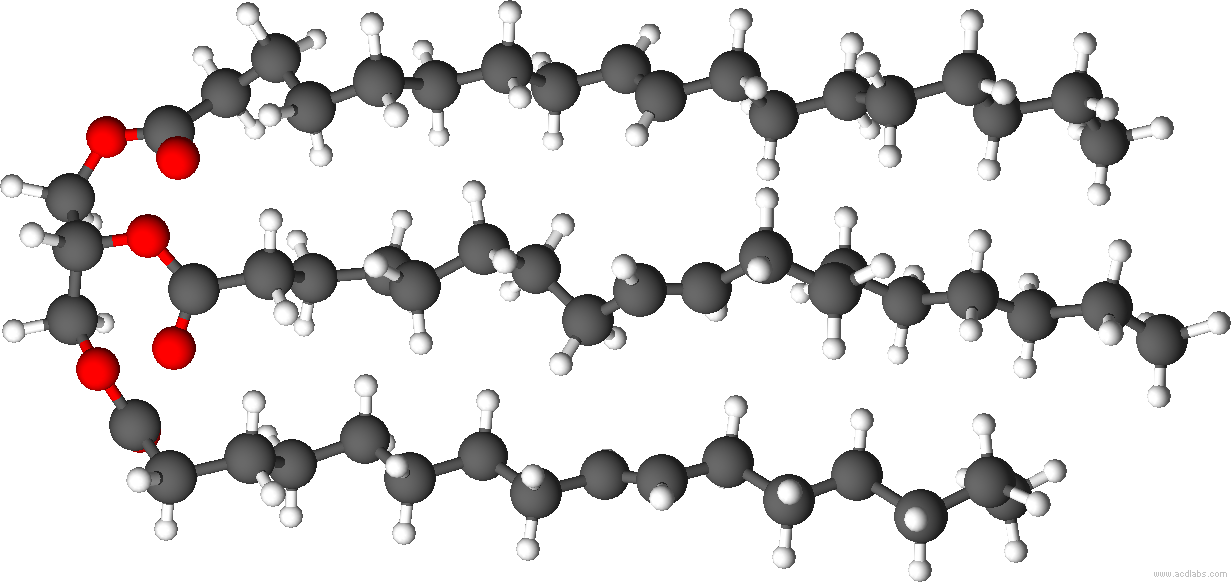
\includegraphics[scale=0.2]{oleine.png}
\caption{Molécule de trioléine de formule $\text{C}_\text{57}\text{H}_\text{104}\text{O}_\text{6}$.}
\label{fig:trioleine}
\end{figure}

La formulation de l'hypothèse concernant la taille d'une molécule d'huile peut être difficile car les élèves ne connaissent a priori pas l'allure de cette molécule, ni même la composition de l'huile.
On peut alors montrer une molécule d'oléine (Fig.~\ref{fig:trioleine}) sous la forme d'une aide ponctuelle apportée au besoin (aide 5 en annexe).
Pour faciliter la représentation dans l'espace de cette molécule, on peut construire un modèle moléculaire (en se limitant par exemple à une molécule de glycérol en indiquant qu'il ne s'agit que d'une partie de la trioléine.
La dimension d'un atome ayant été donnée en cours, on peut alors s'attendre à ce que l'élève compte les atomes qui composent la \og molécule d'huile \fg{} pour estimer sa taille.
Il se pourrait alors que la forme allongée de la molécule induise un questionnement sur la bonne dimension à prendre en compte.
On peut différer la réponse à cette question en attendant de voir ce que donne les résultats des mesures et calculs et en reparler à la fin du TP en s'inspirant des calculs réalisés par Langmuir~\cite{Langmuir1917} : \og D'après vous, comment s'orientent les molécules à la surface de l'eau ? \fg{}.

Après la formulation de l'hypothèse, il est vraisemblable que les élèves soient déstabilisés par le sujet et ne sachent pas comment utiliser les documents pour avancer.
On peut alors apporter une aide sous la forme d'un coup de pouce : \og Déterminer le volume d'une petite cuillère \fg{}.
Ici le choix du verbe \emph{déterminer} me parait plus judicieux que \emph{mesurer} qui limiterait le choix des chemins de résolutions.
On peut en effet s'attendre à ce que l'élève connaisse la valeur du volume d'une petite cuillère, ce qui relève plutôt de la compétence s'approprier et plus particulièrement de la capacité : évaluer quantitativement les grandeurs physiques inconnues et non précisées.\footnote{Les élèves ont fait un exercice leur demandant de relier différents volumes à la contenance de plusieurs récipients, dont un cuillère à café.}
Si la valeur est bonne et que l'élève termine l'activité trop rapidement, on peut toujours l'orienter sur la mesure du volume de la cuillère en l'encourageant à vérifier la valeur utilisée.
Pour la mesure du volume de la cuillère à café, on peut s'attendre à deux méthodes : mesure \og directe \fg{} à l'aide d'une éprouvette graduée ou mesure \og indirecte \fg{} à l'aide d'une balance en passant par la masse volumique.\footnote{La masse volumique a été traitée lors du premier chapitre de l'année.}
Pour ne pas limiter les options des élèves, ils disposent de balances et d'éprouvettes graduées.
Dans les deux cas, l'idée de mesurer le volume de plusieurs cuillerées pour diminuer les incertitudes de mesure pourra être valorisé.

Après avoir déterminé le volume de la petite cuillère, si le groupe est bloqué, il convient d'attirer rapidement l'attention des élèves sur la deuxième grandeur inconnue du sujet : la surface du film d'huile.
\og Dans le sujet, on parle aussi d'une surface : déterminez la valeur de cette surface.\fg{} 
Le calcul de la surface du disque ne doit pas poser problème dans le deuxième cas : la formule est donc rappelée au besoin sans attendre (aide 3 en annexe).
Le schéma du document 2 peut induire un biais : l'étendue de la tache d'huile est simplement repérable par l'absence de vague et pas par sa couleur.
L'épaisseur finale de l'ordre du nanomètre est beaucoup trop faible pour qu'on puisse la repérer optiquement.

Une fois les deux grandeurs déterminées, le lien entre les deux n'est pas forcément limpide.
Les considérations dimensionnelles dépassent pour l'instant les élèves.
Pour aider à faire ce lien, la formule donnant le volume du cylindre est donnée (aide 4 en annexe).
L'attention est portée sur les unités pour éviter de diviser des millilitres par des mètres carrés.

Finalement, le lien entre l'aspect réellement macroscopique de cette expérience et son interprétation microscopique est sans doute une des principales difficultés de cette activité.
Si le lien entre espèce chimique et entité chimique présent dans les programmes a été abordé en cours, il reste flou pour les élèves et il est probable que cette transition gène la conclusion de l'activité.
Le dernier coup de pouce est apporté en ce sens, afin de pousser l'élève à s'interroger sur le résultat obtenu.

\subsection{Analyse a posteriori}

Cette séance a été réalisée à quatre reprises, ce qui a permis d'apporter différentes modifications à l'activité initialement proposée.

En raison notamment des contraintes sanitaires, l'activité était proposée initialement à des binômes libres.
Avec des disparités de niveau importantes, certains groupes avancent plus lentement que d'autres et rares sont ceux qui arrivent à la conclusion de l'activité.
Pour remédier à cela, la dernière séance a été faite avec des trinômes imposés, en tachant de répartir les élèves de manière à obtenir des groupes de niveau plus homogène.
Dans cette configuration, tous les groupes sont parvenus à la conclusion, au moins pour ce qui est du compte-rendu.
Le suivi de la séance est aussi plus facile mais l'individualisation des évaluations est presque impossible puisque les contributions de chacun sont attribuées au groupe.
Les échanges entre les élèves d'un même groupe semblent toutefois très profitables.

Pour la majorité des groupes, l'hypothèse formulée donne le bon ordre de grandeur pour la taille d'une molécule d'huile.
Pour un groupe en particulier, la notion de molécule semble particulièrement déconnectée de l'espèce chimique (\og l'huile \fg{}) : pour eux les petites gouttes d'huile qui tombent lorsqu'on laisse couler doucement l'huile sont des molécules.
Certains groupes confondent molécule et cellule.
Pour d'autres encore, la différence entre atome et molécule n'est pas claire.
Pour ces derniers, la question \og De quoi sont formées les molécules ? \fg{} a généralement suffit pour qu'ils se corrigent eux-même.
En utilisant la représentation de la trioléine, plusieurs groupes comptent tous les atomes composants la molécule ce qui aboutit à une estimation un peu haute de la taille de la molécule : $167 \times \unit{0{,}1}{nm}=\unit{16{,}7}{nm}$.
Certains rapprochent la taille d'une molécule au volume donné comme aide à la conversion : \og La taille d'une molécule d'huile est \unit{1}{mL}. \fg{}.
Il faudrait peut-être modifier la question du sujet pour \og Quelle est la \emph{longueur} d'une molécule d'huile ? \fg{} afin d'éviter cela. 

Après avoir émis leur hypothèse, quelques groupes ($\sim \unit{15}{\%}$) décident eux-même de mesurer l'aire du film d'huile en s'aidant du schéma.
Initialement, l'aide \og Déterminer le volume d'une petite cuillère \fg{} était proposée collectivement.
Pour les groupes mentionnés avant, cette aide n'a aucun sens à ce stade, ce qui justifie d'apporter cette aide ponctuellement.
La majorité des groupes a cependant besoin du coup de pouce pour avancer dans l'activité.
Environ \unit{30}{\%} des élèves sont capables de retrouver la valeur de la contenance d'une petite cuillère sans avoir besoin de faire la mesure.
Pour les autres, la mesure du volume de la cuillère ne pose pas de problème particulier.
Sans doute habitués à avoir sur leur paillasse le matériel nécessaire, certains groupes prennent tout le matériel à leur disposition avant de voir ce dont ils ont réellement besoin pour leur mesure.
La plupart des groupes optent finalement pour une éprouvette graduée.

Lors de la première séance, le deuxième coup de pouce était apporté simplement en distribuant l'aide 4 (Annexe~\ref{ann:aides}) donnant le volume du cylindre.
La plupart des élèves sont alors embrouillés par cette aide qui n'a l'air d'avoir aucun rapport avec le sujet.
Pour les aider à faire le lien lors des séances suivantes, les élèves sont d'abord invités à représenter l'allure de la flaque d'huile en trois dimensions, en perspective.
Il est alors bien plus clair que le cylindre représente le film d'huile.
Souvent à ce stade, les élèves n'ont déterminé que le volume d'huile versé dans l'étang et doivent encore trouver la surface.
Mais dans la formule, il y a aussi $e$ et c'est une longueur qui est affichée sur la vue aérienne de l'étang.
La détermination de la taille de la tache ou de celle de l'étang est parfois difficile : plusieurs fois l'utilisation de l'étalon de longueur n'est pas immédiate.
Elle devient évidente pour eux quand le problème est posé sous la forme d'un produit en croix.
En cela, les critères choisis pour l'évaluation de la compétence réaliser lors de la séance me semble mal gradués et ne rendent pas compte des difficultés réelles des élèves.
Plusieurs groupes ne mesurent pas directement la taille de la tache d'huile mais plutôt celle de l'étang et se reposent sur le texte qui dit que l'huile recouvre un quart de l'étang ce qui parait effectivement plus simple mais que je n'avais pas envisagé initialement.

Avec l'aide 4 (Annexe~\ref{ann:aides}), environ \unit{40}{\%} des élèves parviennent à trouver la bonne valeur pour l'épaisseur du film d'huile.
En revanche un seul élève énonce clairement que l'épaisseur limite du film est dû à la taille des molécules d'huile et que l'épaisseur du film correspond donc à la taille de ces molécules.
Pour les autres, la réponse à la question est simplement donnée comme le résultat du calcul effectué mais sans que les discussions ou les commentaires dans le compte-rendu ne permettent d'affirmer que le lien est établi. 
En classe entière, le retour sur cette conclusion n'a semblé perturber personne.

Lors des recherches biographiques demandées aux élèves, il aurait été intéressant de parler davantage d'Agnes Pockels, notamment pour aborder les questions de diversité dans le monde scientifique.
Cependant, sa contribution à l'expérience, bien qu'essentielle, m'a semblé difficile à expliquer sans rentrer dans les détails de la manipulation réalisée, loin de la simplicité de l'expérience de Benjamin Franklin.

\section*{Conclusion}
\addcontentsline{toc}{section}{Conclusion}

\newpage
\appendix

\bibliography{biblio.bib}
\addcontentsline{toc}{section}{Références}

\newpage
\appendix

\addcontentsline{toc}{section}{Annexes}


\section{Sujet élève}
\label{ann:sujet}

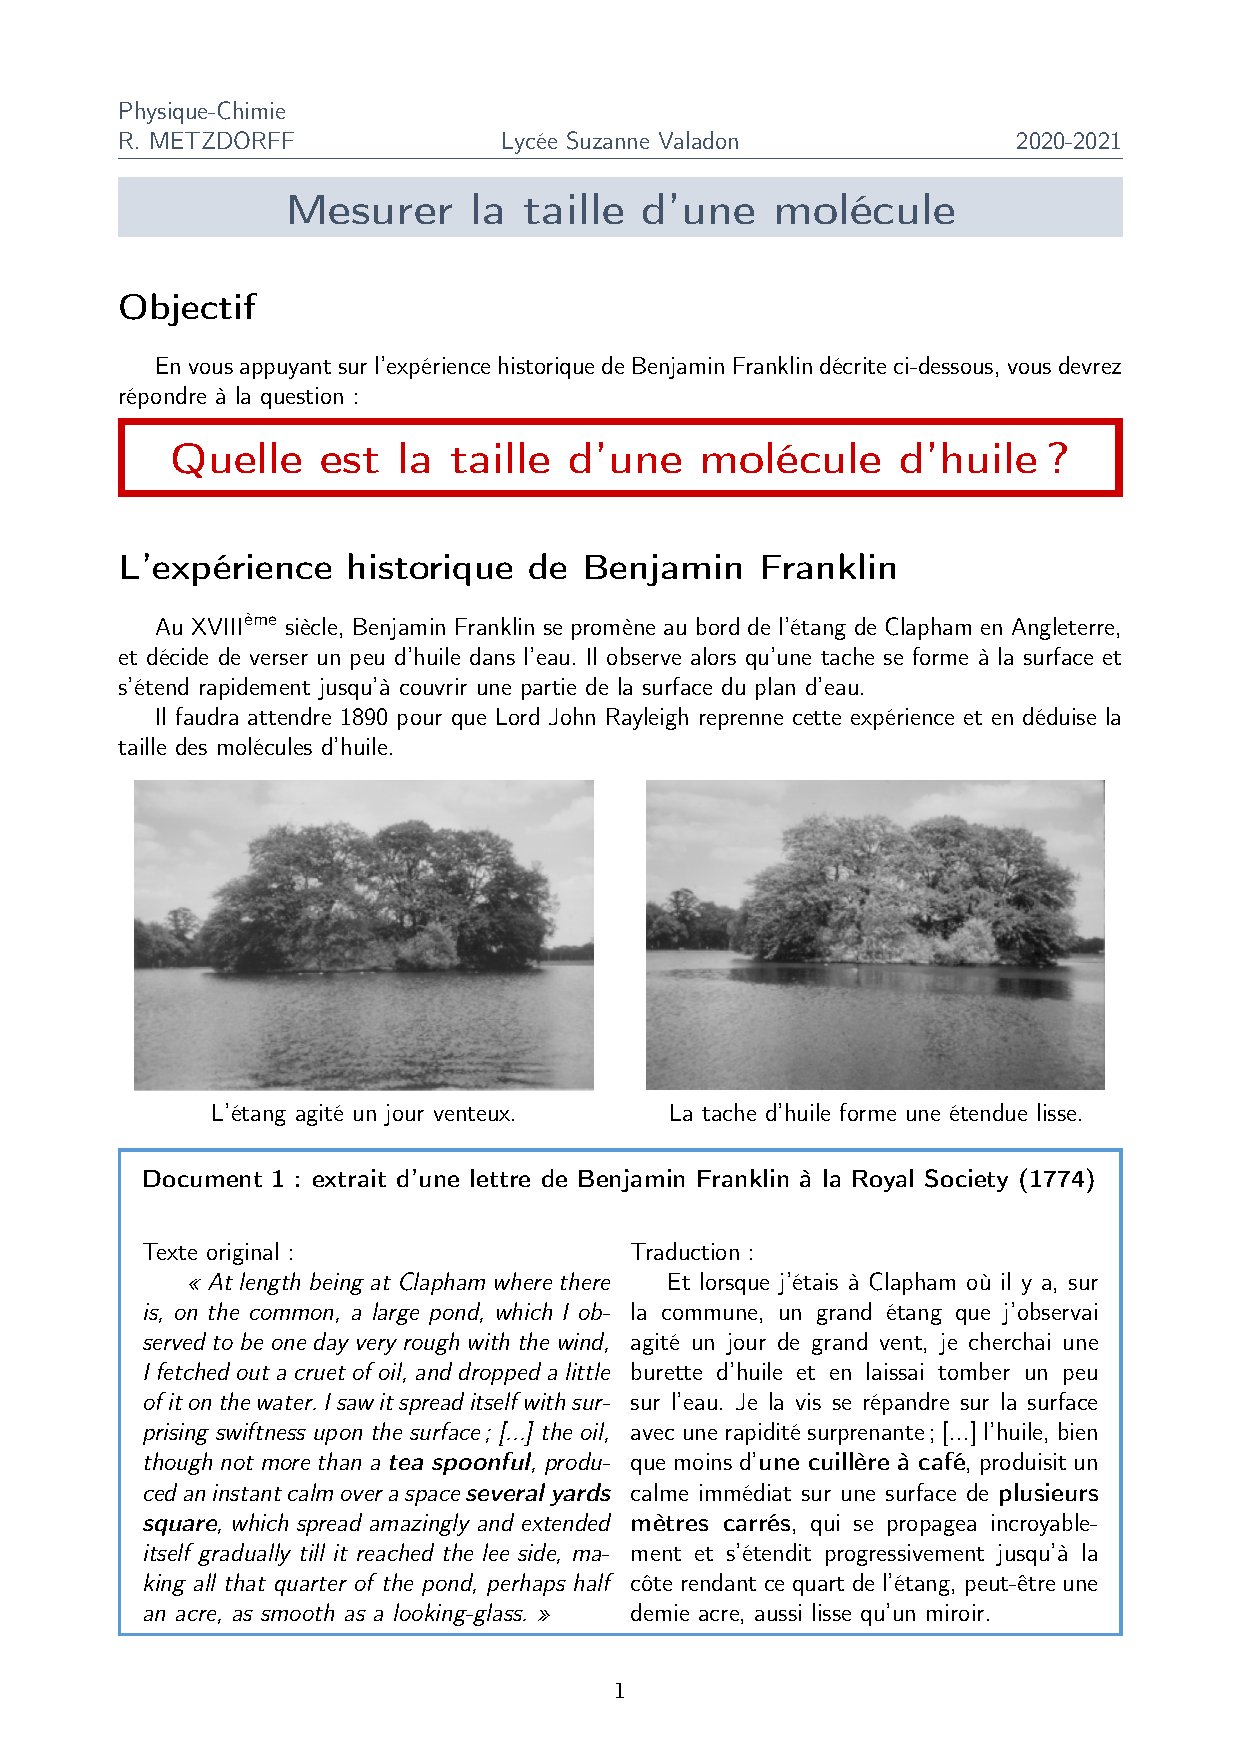
\includepdf[pages=-]{tp_franklin/tp_franklin_v3.pdf}

\section{Aides}
\label{ann:aides}

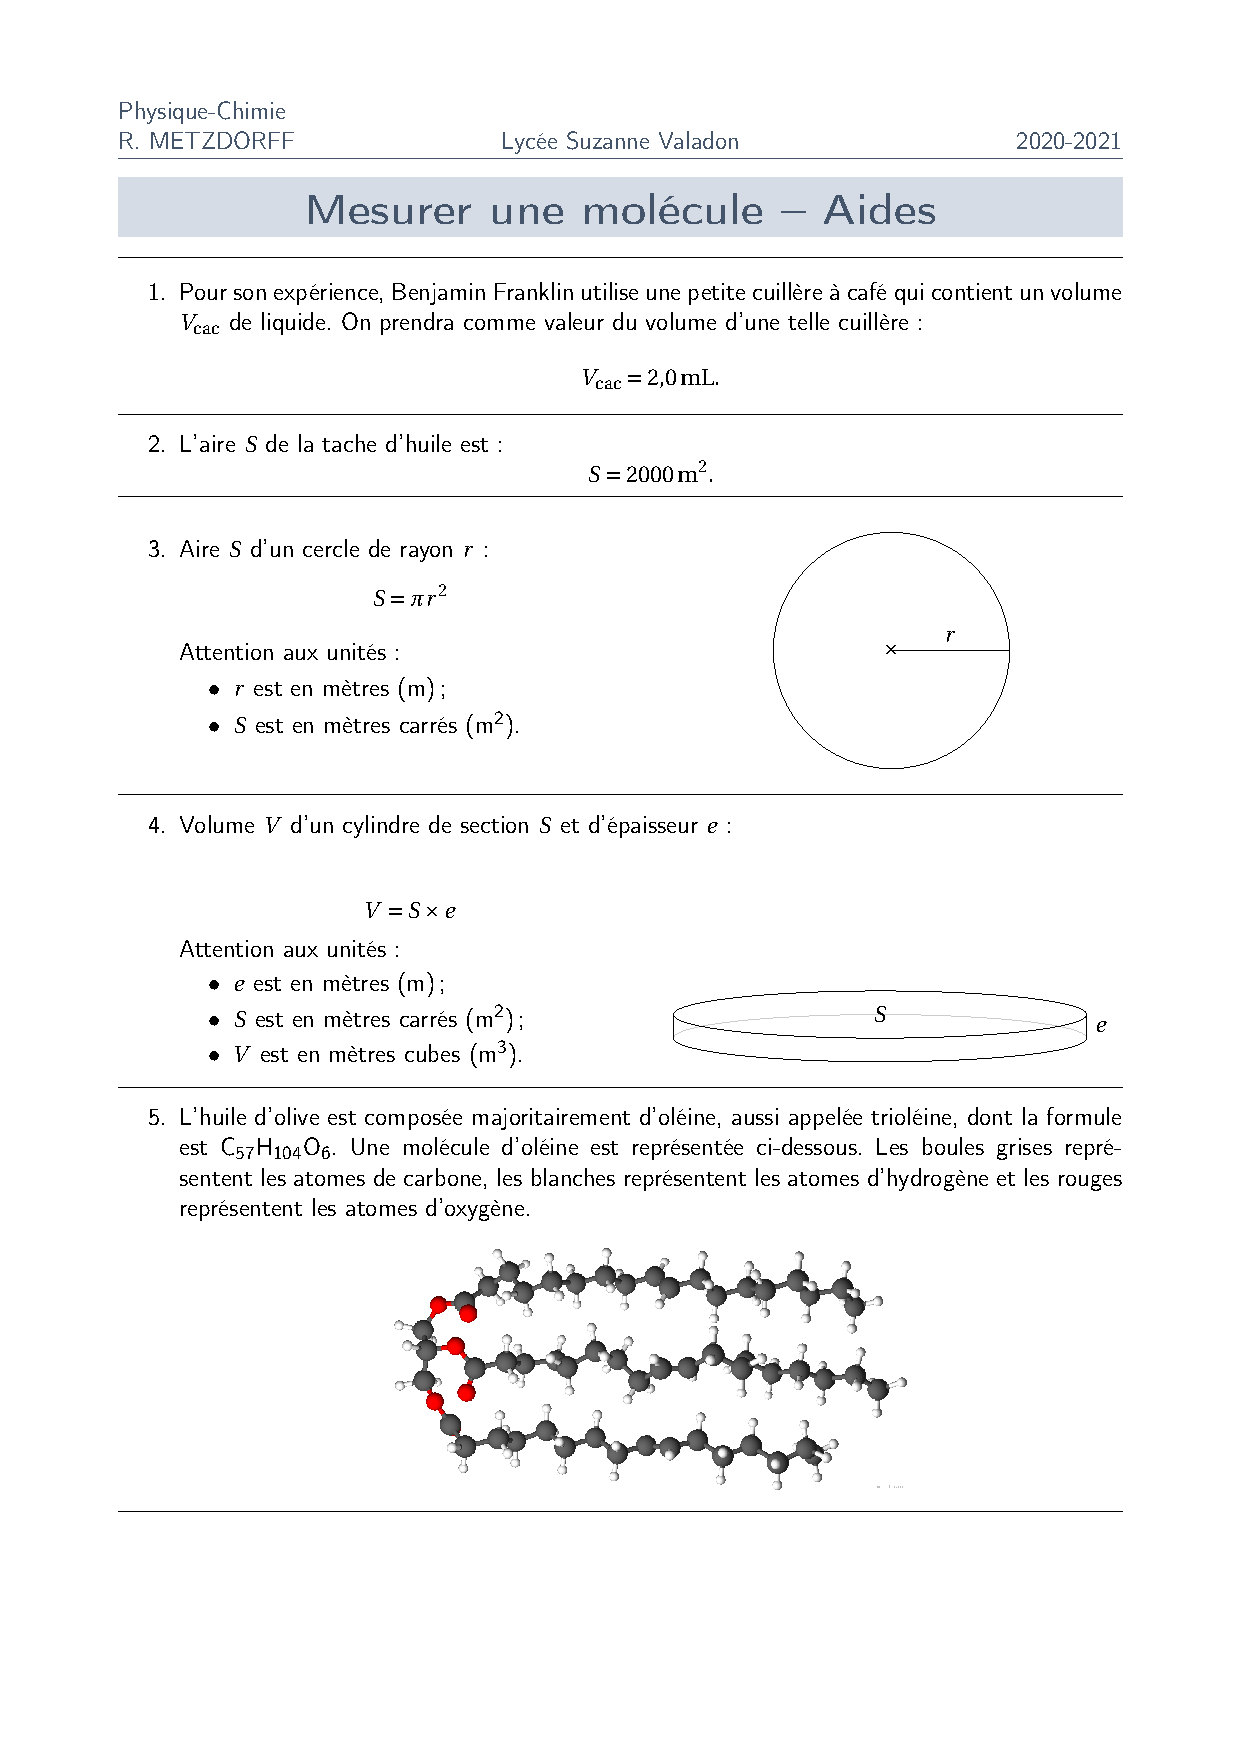
\includepdf[pages=-]{tp_franklin/tp_franklin_aides.pdf}

\section{Fiche de suivi des élèves pendant la séance}

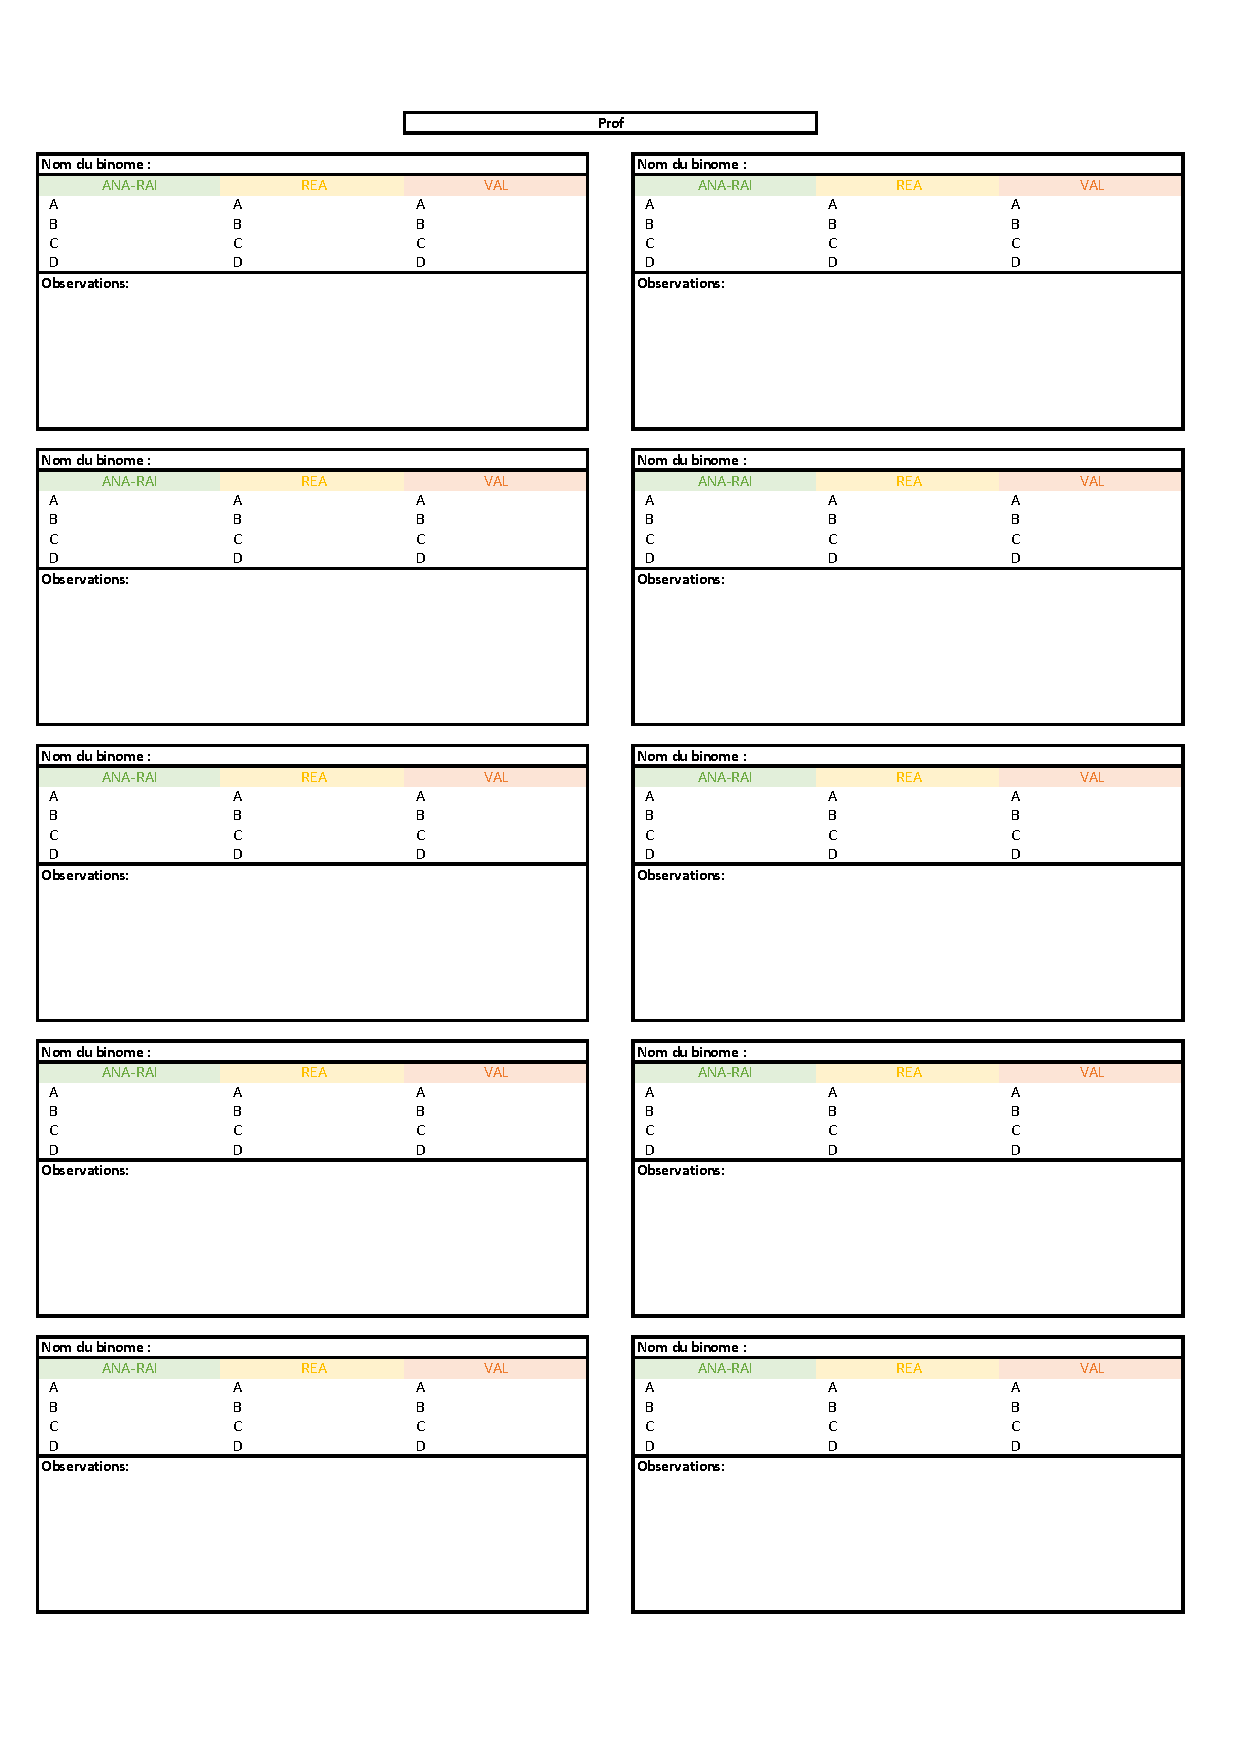
\includepdf[pages=-]{tp_franklin/tp_franklin_prof_suivi-604.pdf}


\end{document}

\begin{center}
\begin{tabular}{l|l}
\textbf{Compétences} & Aptitudes à vérifier \hfill \textbf{Suis-je capable de ... ?} \\
\hline
\hline
\app				 		& Me servir correctement des ressources disponibles (doc, énoncé, ...) \\
		         			& Choisir les informations qui me seront utiles \\
\hline
\anarai		  		& Faire une hypothèse, la justifier \\
							& \textbf{Élaborer un protocole qui répond à la question} \\
      						& Donner des conclusions à l'activité \\
\hline
\rea     				& \textbf{Faire des observations utiles à l'activité} \\
							& Réaliser correctement les calculs analytiques et/ou numériques \\
\hline
\val		      			& Dire si mes résultats sont en accord avec ceux attendus \\
			       			& \textbf{Avoir un regard critique sur mes résultats} \\
\hline
\com				  	& Rendre compte de façon écrite ou orale \\
		         			& Utiliser un vocabulaire et des modes de représentation adaptés \\
\hline
\rco         			& Restituer ses connaissances \\
\end{tabular}
\end{center}

\includepdf[pages=3-11]{../../../biblio/articles/rstl.1774.0044.pdf}
\includepdf[pages=-]{../../../biblio/articles/rspl.1889.0099.pdf}
\includepdf[pages=-]{../../../biblio/articles/pockels_surface_tension.pdf}
\includepdf[pages=2-]{../../../biblio/articles/ajp-jphysrad_1931_2_8_237_0.pdf}
\includepdf[pages=-]{../../../biblio/articles/17_JACS_Langmuir.pdf}
%\includepdf[pages=-]{../../../biblio/articles/}

\newpage
\section{Réalisation expérimentale}

Difficile d'avoir une couche mono-moléculaire.
Il faut :
\begin{itemize}
\item soit un grand étang ;
\item soit une très petite quantité d'huile : il faut la dissoudre dans un solvant volatil.
\end{itemize}
Historiquement, c'est le benzène (appelé benzine à l'époque) mais ça va pas trop toxique.
Dans les protocoles plus modernes, on utilise de l'essence de térébenthine mais ça va pas c'est trop peu volatil et toxique.
Il faudrait essayer l'acétate d'éthyle : aussi volatil que le benzène mais beaucoup moins toxique.
 

\begin{table}
\center
\begin{tabular}{l|c|l}
\textbf{Composé} & $P_\mathrm{sat}^{\unit{20}{\celsius}}$ (mbar) & \textbf{Toxicité} \\
\hline \hline
Éther diéthylique & 586 & H224, H302, H336 \\
Cyclohexane & 127 & H225, H304, H315, H336, H410 \\
Benzène & 100 & H225, H304, H315, H319, H340, H350, H372 \\
Acétate d'éthyle & 100 & H225, H319, H336 \\
Éthanol & 58 & H225 \\
Toluène & 29 & H225, H304, H315, H336, H361d, H373 \\
Essence de térébenthine  & 5{,}35 &  H226, H302, H304, H312, H315, H317, H319, ... \\
\end{tabular}
\caption{Éther diéthylique : trop inflammable. Cyclohexane : trop toxique. Benzène : trop toxique. Acétate d'éthyle : soluble dans l'eau. Éthanol : soluble dans l'eau, a priori huile non soluble dedans, seulement l'acide oléique. Essence de térébenthine : peu volatil et toxique. Toluène : actuellement utilisé comme substitut au benzène.}
\end{table}